\documentclass[../experiment.tex]{subfiles}
\graphicspath{{\subfix{../../../images/}}}
\begin{document}
    \textbf{Lithium metasilicate}, also known as lithium silicate monohydrate, is a compound with the chemical 
    formula $Li_2SiO_3·H_{2}O$. It consists of lithium ($Li$) cations, silicate ($SiO_3$) anions, and one water 
    molecule ($H_2O$) per formula unit.It is typically encountered as a white crystalline powder or granules. 
    Its physical properties, such as density and melting point, can vary depending on factors such as crystal 
    structure and the presence of impurities.These materials have physicochemical stability at high temperatures, 
    compatibility with other types of structural materials, radiation stability and adequate heat transfer. The 
    main feature is their high sensitivity to ionizing radiation for a wide energy range. Also, $Li_2SiO_3$ 
    ($Z_{eff} = 10.5$) being low Z materials, are near tissue equivalent and may find application in the field of 
    radiation dosimetry\cite{a11}. 

    \subsubsection{Synthesis of $Li_2SiO_3$ (pure)}
        Lithium metasilicate was prepared by soild state reaction method\cite{a14} using the following chemical reaction.
        \begin{center}
            \ch{Li2CO3 + SiO2 -> Li2SiO3 + CO2}
        \end{center}

        To synthesize Lithium metasilicate 5g of $Li_2CO_3$ and 4.065g of $SiO_2$ was measured and grinded using 
        a mortar and pestle with the addition of acetone for 30 minutes to form a smooth white paste. This paste
        was then heated in a heating mantle for 30 minutes to let the acetone evaporate out. The residual solid was 
        then grounded to a fine powder using mortar and pestle. The sample was then heated in a muffle furnace at 
        $900^{\circ}C$ for 4 hours in air and then cooled down to room temperature. The resulting sample was grounded 
        again for 30 minutes using mortar and pestle.
        \FloatBarrier\begin{multicols}{2}
            \begin{Figure}
                \centering
                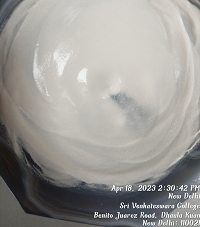
\includegraphics[width=0.6\linewidth]{d1.png}
                \captionof{figure}{Precursor materials being weighed and grounded into a fine paste with acetone}\label{fig:d1}
            \end{Figure}
            \begin{Figure}
                \centering
                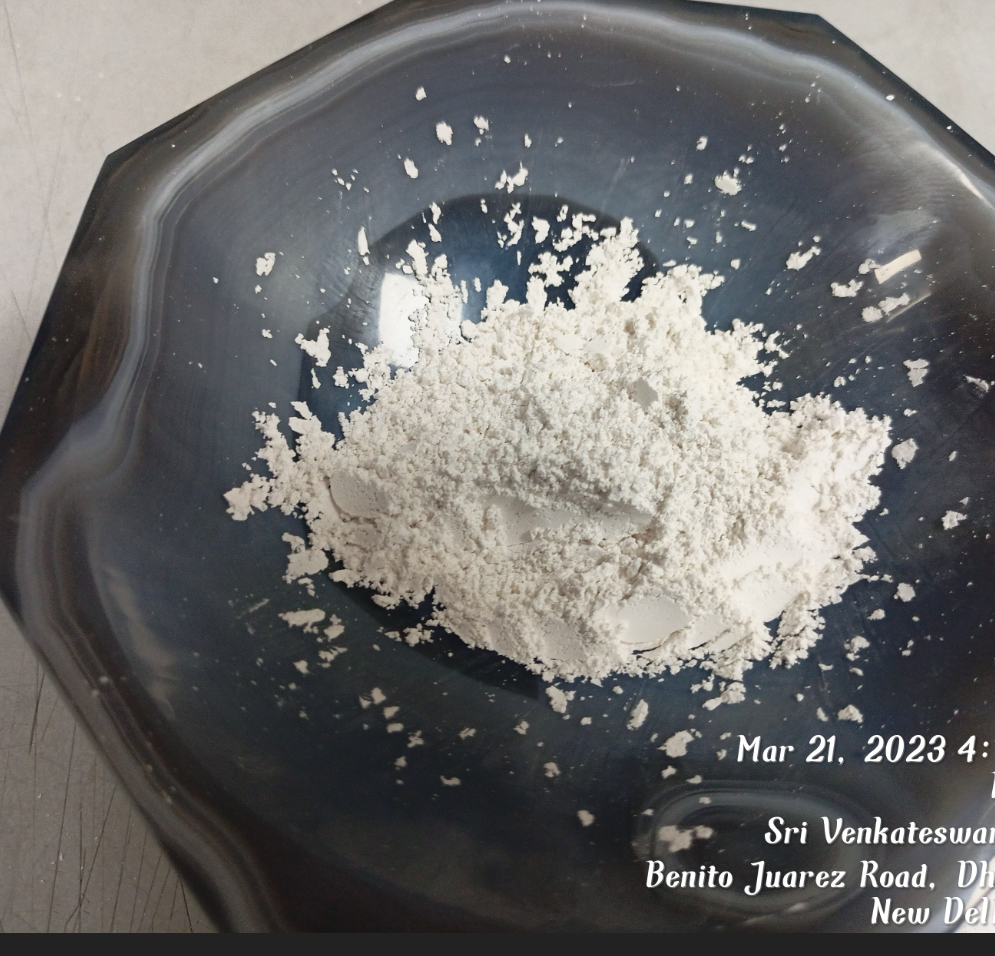
\includegraphics[width=0.6\linewidth]{d2.png}
                \captionof{figure}{Sample being ground after removing acetone by heating with heating mantle}\label{fig:d2}
            \end{Figure}  
        \end{multicols}
    \subsubsection{Dopant Optimization for $Li_2SiO_3$}
        To study the effect of doping on the thermoluminescence of the given sample, $Li_2SiO_3$ is prepared using 
        solid state reaction method under the same conditions but the samples are being doped with 5 rare earth metals.
        $Li_2SiO_3$ was doped with Dysprosium, Europium, Terbium, Erbium and Cerium at 0.1 mol\%. The chemical reaction for 
        the process is given below:
        \begin{center}
            \ch{Li2CO3 + SiO2 ->[$X^{3+}$ (0.1 mol\%)] Li2SiO3:X + CO2}
        \end{center}
        where X is the dopant material, for example Dysprosium, Europium, Terbium, Erbium or Cerium
        To synthesize doped Lithium metasilicate 4.99g of $Li_2CO_3$ and 4.065g of $SiO_2$ along with calculated 
        amount of rare earth metals was measured and grinded using a mortar and pestle with the addition of 
        acetone for 30 minutes to form a smooth white paste. This paste was then heated in a heating mantle for 
        30 minutes to let the acetone evaporate out. The residual solid was then grounded to a fine powder using 
        mortar and pestle. The sample was then heated in a muffle furnace at $900^{\circ}C$ for 4 hours in air and 
        then cooled down to room temperature. The resulting sample was grounded again for 30 minutes using mortar and pestle.
        \FloatBarrier\begin{multicols}{2}
            \begin{Figure}
                \centering
                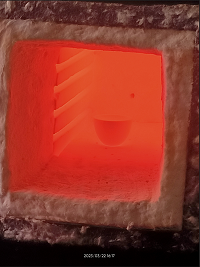
\includegraphics[width=0.5\linewidth]{d3.png}
                \captionof{figure}{Sample being annealed in a furnace at $900^{\circ}C$ for 4 hours}\label{fig:d3}
            \end{Figure}
            \begin{Figure}
                \centering
                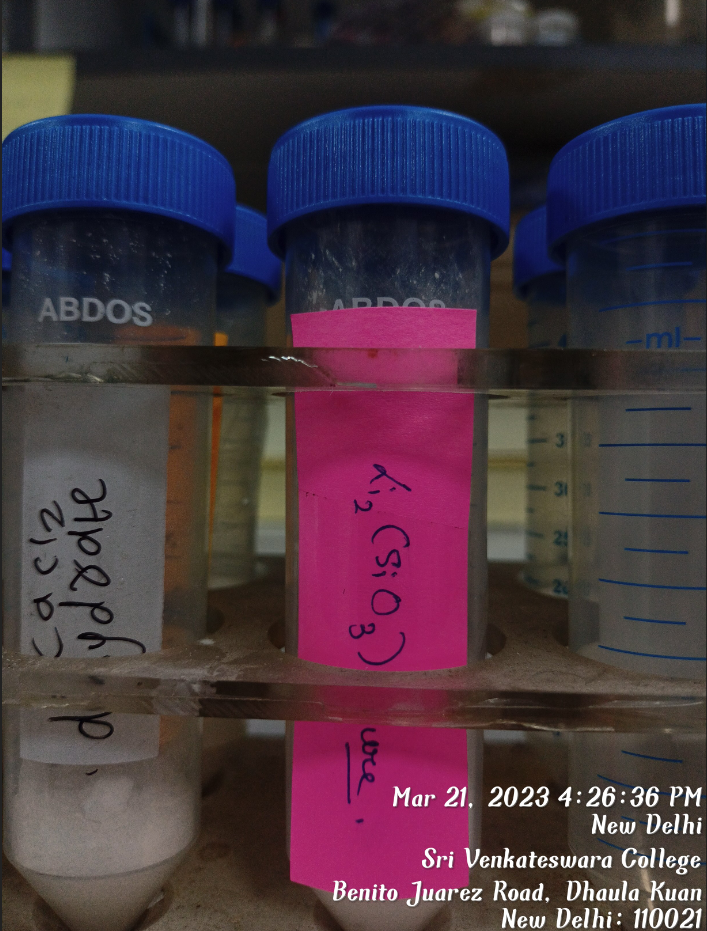
\includegraphics[width=0.5\linewidth]{d4.png}
                \captionof{figure}{Final sample after preparation}\label{fig:d4}
            \end{Figure}
        \end{multicols}
        
\end{document}